% !TEX TS-program = pdflatex
% !TEX encoding = UTF-8 Unicode
\documentclass[border=0mm]{standalone}
% packages
\usepackage{tikz}
\usetikzlibrary{patterns}
\usepackage{amsmath,amssymb}
\usepackage{bm}
\usepackage{pgfplots}
\pgfplotsset{compat=1.15}
% start document
\begin{document}
% generated by ROOT (CERN)
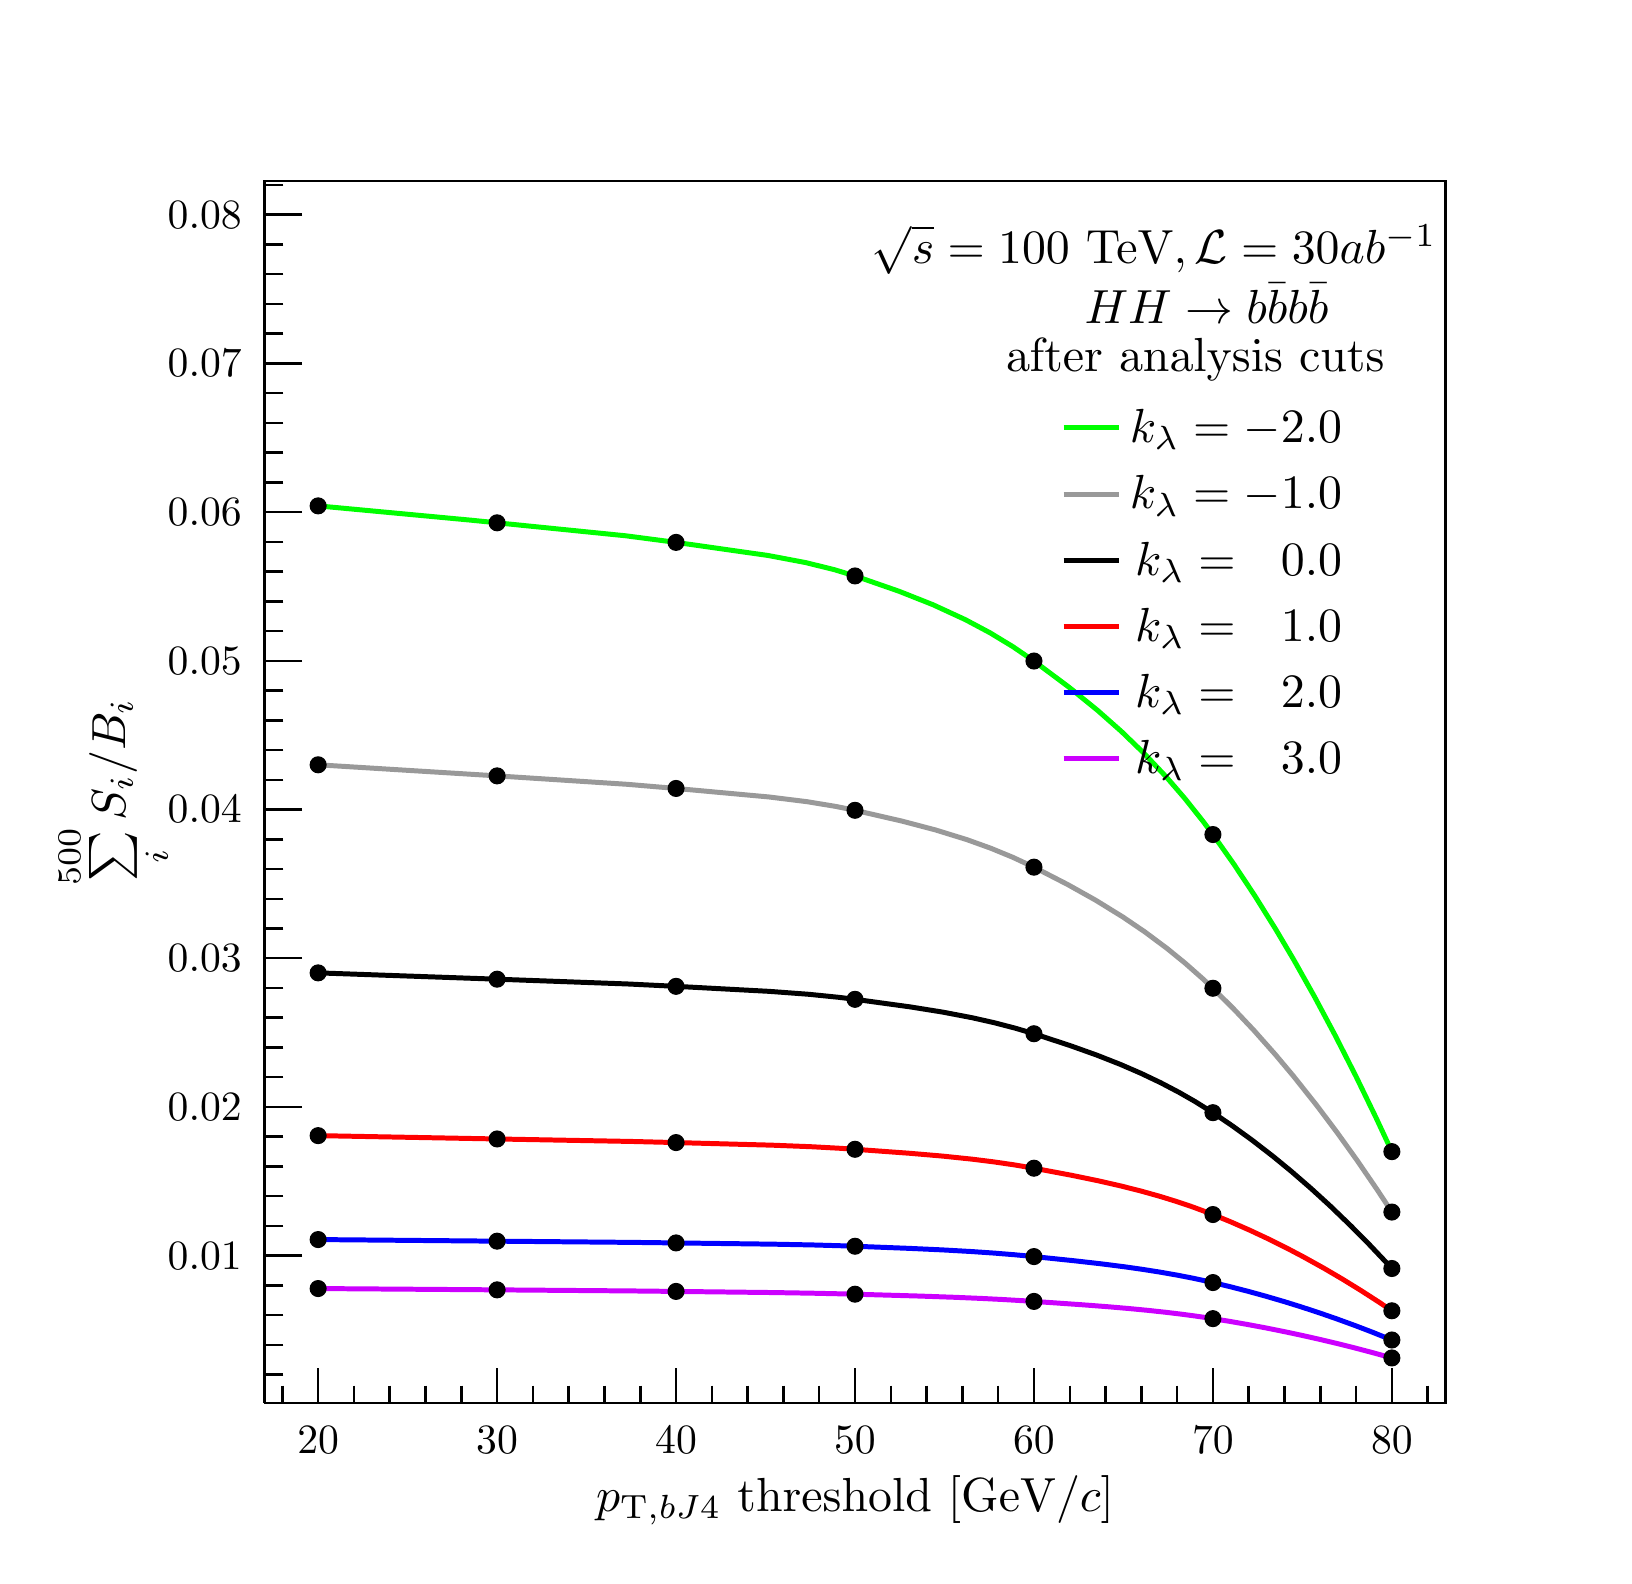
\begin{tikzpicture}
\pgfdeclareplotmark{cross} {
\pgfpathmoveto{\pgfpoint{-0.3\pgfplotmarksize}{\pgfplotmarksize}}
\pgfpathlineto{\pgfpoint{+0.3\pgfplotmarksize}{\pgfplotmarksize}}
\pgfpathlineto{\pgfpoint{+0.3\pgfplotmarksize}{0.3\pgfplotmarksize}}
\pgfpathlineto{\pgfpoint{+1\pgfplotmarksize}{0.3\pgfplotmarksize}}
\pgfpathlineto{\pgfpoint{+1\pgfplotmarksize}{-0.3\pgfplotmarksize}}
\pgfpathlineto{\pgfpoint{+0.3\pgfplotmarksize}{-0.3\pgfplotmarksize}}
\pgfpathlineto{\pgfpoint{+0.3\pgfplotmarksize}{-1.\pgfplotmarksize}}
\pgfpathlineto{\pgfpoint{-0.3\pgfplotmarksize}{-1.\pgfplotmarksize}}
\pgfpathlineto{\pgfpoint{-0.3\pgfplotmarksize}{-0.3\pgfplotmarksize}}
\pgfpathlineto{\pgfpoint{-1.\pgfplotmarksize}{-0.3\pgfplotmarksize}}
\pgfpathlineto{\pgfpoint{-1.\pgfplotmarksize}{0.3\pgfplotmarksize}}
\pgfpathlineto{\pgfpoint{-0.3\pgfplotmarksize}{0.3\pgfplotmarksize}}
\pgfpathclose
\pgfusepathqstroke
}
\pgfdeclareplotmark{cross*} {
\pgfpathmoveto{\pgfpoint{-0.3\pgfplotmarksize}{\pgfplotmarksize}}
\pgfpathlineto{\pgfpoint{+0.3\pgfplotmarksize}{\pgfplotmarksize}}
\pgfpathlineto{\pgfpoint{+0.3\pgfplotmarksize}{0.3\pgfplotmarksize}}
\pgfpathlineto{\pgfpoint{+1\pgfplotmarksize}{0.3\pgfplotmarksize}}
\pgfpathlineto{\pgfpoint{+1\pgfplotmarksize}{-0.3\pgfplotmarksize}}
\pgfpathlineto{\pgfpoint{+0.3\pgfplotmarksize}{-0.3\pgfplotmarksize}}
\pgfpathlineto{\pgfpoint{+0.3\pgfplotmarksize}{-1.\pgfplotmarksize}}
\pgfpathlineto{\pgfpoint{-0.3\pgfplotmarksize}{-1.\pgfplotmarksize}}
\pgfpathlineto{\pgfpoint{-0.3\pgfplotmarksize}{-0.3\pgfplotmarksize}}
\pgfpathlineto{\pgfpoint{-1.\pgfplotmarksize}{-0.3\pgfplotmarksize}}
\pgfpathlineto{\pgfpoint{-1.\pgfplotmarksize}{0.3\pgfplotmarksize}}
\pgfpathlineto{\pgfpoint{-0.3\pgfplotmarksize}{0.3\pgfplotmarksize}}
\pgfpathclose
\pgfusepathqfillstroke
}
\pgfdeclareplotmark{newstar} {
\pgfpathmoveto{\pgfqpoint{0pt}{\pgfplotmarksize}}
\pgfpathlineto{\pgfqpointpolar{44}{0.5\pgfplotmarksize}}
\pgfpathlineto{\pgfqpointpolar{18}{\pgfplotmarksize}}
\pgfpathlineto{\pgfqpointpolar{-20}{0.5\pgfplotmarksize}}
\pgfpathlineto{\pgfqpointpolar{-54}{\pgfplotmarksize}}
\pgfpathlineto{\pgfqpointpolar{-90}{0.5\pgfplotmarksize}}
\pgfpathlineto{\pgfqpointpolar{234}{\pgfplotmarksize}}
\pgfpathlineto{\pgfqpointpolar{198}{0.5\pgfplotmarksize}}
\pgfpathlineto{\pgfqpointpolar{162}{\pgfplotmarksize}}
\pgfpathlineto{\pgfqpointpolar{134}{0.5\pgfplotmarksize}}
\pgfpathclose
\pgfusepathqstroke
}
\pgfdeclareplotmark{newstar*} {
\pgfpathmoveto{\pgfqpoint{0pt}{\pgfplotmarksize}}
\pgfpathlineto{\pgfqpointpolar{44}{0.5\pgfplotmarksize}}
\pgfpathlineto{\pgfqpointpolar{18}{\pgfplotmarksize}}
\pgfpathlineto{\pgfqpointpolar{-20}{0.5\pgfplotmarksize}}
\pgfpathlineto{\pgfqpointpolar{-54}{\pgfplotmarksize}}
\pgfpathlineto{\pgfqpointpolar{-90}{0.5\pgfplotmarksize}}
\pgfpathlineto{\pgfqpointpolar{234}{\pgfplotmarksize}}
\pgfpathlineto{\pgfqpointpolar{198}{0.5\pgfplotmarksize}}
\pgfpathlineto{\pgfqpointpolar{162}{\pgfplotmarksize}}
\pgfpathlineto{\pgfqpointpolar{134}{0.5\pgfplotmarksize}}
\pgfpathclose
\pgfusepathqfillstroke
}
\definecolor{c}{rgb}{1,1,1};
\draw [color=c, fill=c] (0,0) rectangle (20,19.397);
\draw [color=c, fill=c] (3,1.9397) rectangle (18,17.4573);
\definecolor{c}{rgb}{0,0,0};
\draw [c,line width=0.9] (3,1.9397) -- (3,17.4573) -- (18,17.4573) -- (18,1.9397) -- (3,1.9397);
\definecolor{c}{rgb}{1,1,1};
\draw [color=c, fill=c] (3,1.9397) rectangle (18,17.4573);
\definecolor{c}{rgb}{0,0,0};
\draw [c,line width=0.9] (3,1.9397) -- (3,17.4573) -- (18,17.4573) -- (18,1.9397) -- (3,1.9397);
\draw [c,line width=0.9] (3,1.9397) -- (18,1.9397);
\draw [c,line width=0.9] (3.68182,2.37613) -- (3.68182,1.9397);
\draw [c,line width=0.9] (4.13636,2.15791) -- (4.13636,1.9397);
\draw [c,line width=0.9] (4.59091,2.15791) -- (4.59091,1.9397);
\draw [c,line width=0.9] (5.04545,2.15791) -- (5.04545,1.9397);
\draw [c,line width=0.9] (5.5,2.15791) -- (5.5,1.9397);
\draw [c,line width=0.9] (5.95455,2.37613) -- (5.95455,1.9397);
\draw [c,line width=0.9] (6.40909,2.15791) -- (6.40909,1.9397);
\draw [c,line width=0.9] (6.86364,2.15791) -- (6.86364,1.9397);
\draw [c,line width=0.9] (7.31818,2.15791) -- (7.31818,1.9397);
\draw [c,line width=0.9] (7.77273,2.15791) -- (7.77273,1.9397);
\draw [c,line width=0.9] (8.22727,2.37613) -- (8.22727,1.9397);
\draw [c,line width=0.9] (8.68182,2.15791) -- (8.68182,1.9397);
\draw [c,line width=0.9] (9.13636,2.15791) -- (9.13636,1.9397);
\draw [c,line width=0.9] (9.59091,2.15791) -- (9.59091,1.9397);
\draw [c,line width=0.9] (10.0455,2.15791) -- (10.0455,1.9397);
\draw [c,line width=0.9] (10.5,2.37613) -- (10.5,1.9397);
\draw [c,line width=0.9] (10.9545,2.15791) -- (10.9545,1.9397);
\draw [c,line width=0.9] (11.4091,2.15791) -- (11.4091,1.9397);
\draw [c,line width=0.9] (11.8636,2.15791) -- (11.8636,1.9397);
\draw [c,line width=0.9] (12.3182,2.15791) -- (12.3182,1.9397);
\draw [c,line width=0.9] (12.7727,2.37613) -- (12.7727,1.9397);
\draw [c,line width=0.9] (13.2273,2.15791) -- (13.2273,1.9397);
\draw [c,line width=0.9] (13.6818,2.15791) -- (13.6818,1.9397);
\draw [c,line width=0.9] (14.1364,2.15791) -- (14.1364,1.9397);
\draw [c,line width=0.9] (14.5909,2.15791) -- (14.5909,1.9397);
\draw [c,line width=0.9] (15.0455,2.37613) -- (15.0455,1.9397);
\draw [c,line width=0.9] (15.5,2.15791) -- (15.5,1.9397);
\draw [c,line width=0.9] (15.9545,2.15791) -- (15.9545,1.9397);
\draw [c,line width=0.9] (16.4091,2.15791) -- (16.4091,1.9397);
\draw [c,line width=0.9] (16.8636,2.15791) -- (16.8636,1.9397);
\draw [c,line width=0.9] (17.3182,2.37613) -- (17.3182,1.9397);
\draw [c,line width=0.9] (3.68182,2.37613) -- (3.68182,1.9397);
\draw [c,line width=0.9] (3.22727,2.15791) -- (3.22727,1.9397);
\draw [c,line width=0.9] (17.3182,2.37613) -- (17.3182,1.9397);
\draw [c,line width=0.9] (17.7727,2.15791) -- (17.7727,1.9397);
\draw [anchor=base] (3.68182,1.2996) node[scale=1.50669, color=c, rotate=0]{20};
\draw [anchor=base] (5.95455,1.2996) node[scale=1.50669, color=c, rotate=0]{30};
\draw [anchor=base] (8.22727,1.2996) node[scale=1.50669, color=c, rotate=0]{40};
\draw [anchor=base] (10.5,1.2996) node[scale=1.50669, color=c, rotate=0]{50};
\draw [anchor=base] (12.7727,1.2996) node[scale=1.50669, color=c, rotate=0]{60};
\draw [anchor=base] (15.0455,1.2996) node[scale=1.50669, color=c, rotate=0]{70};
\draw [anchor=base] (17.3182,1.2996) node[scale=1.50669, color=c, rotate=0]{80};
\draw (10.5,0.698292) node[scale=1.7299, color=c, rotate=0]{$p_{\text{T},bJ4} \text{~threshold} ~[\text{GeV}/c]$};
\draw [c,line width=0.9] (3,1.9397) -- (3,17.4573);
\draw [c,line width=0.9] (3.48,3.80895) -- (3,3.80895);
\draw [c,line width=0.9] (3.24,4.18664) -- (3,4.18664);
\draw [c,line width=0.9] (3.24,4.56433) -- (3,4.56433);
\draw [c,line width=0.9] (3.24,4.94202) -- (3,4.94202);
\draw [c,line width=0.9] (3.24,5.31971) -- (3,5.31971);
\draw [c,line width=0.9] (3.48,5.6974) -- (3,5.6974);
\draw [c,line width=0.9] (3.24,6.0751) -- (3,6.0751);
\draw [c,line width=0.9] (3.24,6.45279) -- (3,6.45279);
\draw [c,line width=0.9] (3.24,6.83048) -- (3,6.83048);
\draw [c,line width=0.9] (3.24,7.20817) -- (3,7.20817);
\draw [c,line width=0.9] (3.48,7.58586) -- (3,7.58586);
\draw [c,line width=0.9] (3.24,7.96355) -- (3,7.96355);
\draw [c,line width=0.9] (3.24,8.34124) -- (3,8.34124);
\draw [c,line width=0.9] (3.24,8.71893) -- (3,8.71893);
\draw [c,line width=0.9] (3.24,9.09662) -- (3,9.09662);
\draw [c,line width=0.9] (3.48,9.47431) -- (3,9.47431);
\draw [c,line width=0.9] (3.24,9.85201) -- (3,9.85201);
\draw [c,line width=0.9] (3.24,10.2297) -- (3,10.2297);
\draw [c,line width=0.9] (3.24,10.6074) -- (3,10.6074);
\draw [c,line width=0.9] (3.24,10.9851) -- (3,10.9851);
\draw [c,line width=0.9] (3.48,11.3628) -- (3,11.3628);
\draw [c,line width=0.9] (3.24,11.7405) -- (3,11.7405);
\draw [c,line width=0.9] (3.24,12.1182) -- (3,12.1182);
\draw [c,line width=0.9] (3.24,12.4958) -- (3,12.4958);
\draw [c,line width=0.9] (3.24,12.8735) -- (3,12.8735);
\draw [c,line width=0.9] (3.48,13.2512) -- (3,13.2512);
\draw [c,line width=0.9] (3.24,13.6289) -- (3,13.6289);
\draw [c,line width=0.9] (3.24,14.0066) -- (3,14.0066);
\draw [c,line width=0.9] (3.24,14.3843) -- (3,14.3843);
\draw [c,line width=0.9] (3.24,14.762) -- (3,14.762);
\draw [c,line width=0.9] (3.48,15.1397) -- (3,15.1397);
\draw [c,line width=0.9] (3.24,15.5174) -- (3,15.5174);
\draw [c,line width=0.9] (3.24,15.8951) -- (3,15.8951);
\draw [c,line width=0.9] (3.24,16.2728) -- (3,16.2728);
\draw [c,line width=0.9] (3.24,16.6504) -- (3,16.6504);
\draw [c,line width=0.9] (3.48,17.0281) -- (3,17.0281);
\draw [c,line width=0.9] (3.48,3.80895) -- (3,3.80895);
\draw [c,line width=0.9] (3.24,3.43126) -- (3,3.43126);
\draw [c,line width=0.9] (3.24,3.05357) -- (3,3.05357);
\draw [c,line width=0.9] (3.24,2.67588) -- (3,2.67588);
\draw [c,line width=0.9] (3.24,2.29819) -- (3,2.29819);
\draw [c,line width=0.9] (3.48,17.0281) -- (3,17.0281);
\draw [c,line width=0.9] (3.24,17.4058) -- (3,17.4058);
\draw [anchor= east] (2.9,3.80895) node[scale=1.50669, color=c, rotate=0]{0.01};
\draw [anchor= east] (2.9,5.6974) node[scale=1.50669, color=c, rotate=0]{0.02};
\draw [anchor= east] (2.9,7.58586) node[scale=1.50669, color=c, rotate=0]{0.03};
\draw [anchor= east] (2.9,9.47431) node[scale=1.50669, color=c, rotate=0]{0.04};
\draw [anchor= east] (2.9,11.3628) node[scale=1.50669, color=c, rotate=0]{0.05};
\draw [anchor= east] (2.9,13.2512) node[scale=1.50669, color=c, rotate=0]{0.06};
\draw [anchor= east] (2.9,15.1397) node[scale=1.50669, color=c, rotate=0]{0.07};
\draw [anchor= east] (2.9,17.0281) node[scale=1.50669, color=c, rotate=0]{0.08};
\draw (1.08,9.69849) node[scale=1.7299, color=c, rotate=90]{$\sum\limits_{i}^{500} S_{i}/B_{i}$};
\definecolor{c}{rgb}{0,1,0};
\draw [c,line width=1.8] (3.68182,13.3308) -- (5.63632,13.1478) -- (5.95455,13.1156) -- (7.58918,12.9507) -- (8.22727,12.867) -- (9.39637,12.7006) -- (9.87484,12.6102) -- (10.2354,12.5212) -- (10.5,12.4408) -- (11.0615,12.2454) -- (11.4904,12.0753)
 -- (11.901,11.886) -- (12.2145,11.7189) -- (12.5032,11.5441) -- (12.7727,11.3603) -- (13.221,11.0254) -- (13.5806,10.7337) -- (13.8845,10.4647) -- (14.1678,10.1907) -- (14.4552,9.88586) -- (14.6865,9.61796) -- (14.9187,9.32635) -- (15.0455,9.15683)
 -- (15.3117,8.78021) -- (15.5768,8.38013) -- (15.8449,7.95025) -- (16.073,7.56443) -- (16.3363,7.09602) -- (16.6008,6.60031) -- (16.8632,6.08375) -- (17.1192,5.55593) -- (17.3182,5.12934);
\definecolor{c}{rgb}{0,0,0};
\foreach \P in {(3.68182,13.3308), (5.95455,13.1156), (8.22727,12.867), (10.5,12.4408), (12.7727,11.3603), (15.0455,9.15683), (17.3182,5.12934)}{\draw[mark options={color=c,fill=c},mark size=2.882883pt,mark=*] plot coordinates {\P};}
\definecolor{c}{rgb}{0.6,0.6,0.6};
\draw [c,line width=1.8] (3.68182,10.0424) -- (5.95455,9.90168) -- (7.60375,9.79484) -- (8.22727,9.74201) -- (9.40937,9.63359) -- (9.8896,9.57409) -- (10.2539,9.51432) -- (10.5,9.46452) -- (11.0949,9.32774) -- (11.5195,9.21594) -- (11.9203,9.09222)
 -- (12.2251,8.9825) -- (12.5035,8.86796) -- (12.7727,8.7422) -- (13.2048,8.51971) -- (13.5574,8.32213) -- (13.9021,8.1096) -- (14.1794,7.92138) -- (14.4629,7.71013) -- (14.691,7.52441) -- (14.9202,7.32215) -- (15.0455,7.20439) -- (15.3074,6.94394)
 -- (15.5686,6.66689) -- (15.8379,6.36317) -- (16.0669,6.0904) -- (16.3601,5.72158) -- (16.6203,5.3758) -- (16.8774,5.01712) -- (17.1299,4.6482) -- (17.3182,4.36233);
\definecolor{c}{rgb}{0,0,0};
\foreach \P in {(3.68182,10.0424), (5.95455,9.90168), (8.22727,9.74201), (10.5,9.46452), (12.7727,8.7422), (15.0455,7.20439), (17.3182,4.36233)}{\draw[mark options={color=c,fill=c},mark size=2.882883pt,mark=*] plot coordinates {\P};}
\draw [c,line width=1.8] (3.68182,7.39989) -- (5.95455,7.31969) -- (7.62065,7.25863) -- (8.22727,7.2288) -- (9.41412,7.16494) -- (9.91109,7.128) -- (10.2927,7.08968) -- (10.5,7.06412) -- (11.1992,6.96816) -- (11.6116,6.9021) -- (11.9853,6.83078) --
 (12.2725,6.76602) -- (12.5403,6.69611) -- (12.7727,6.6269) -- (13.227,6.47817) -- (13.5725,6.3547) -- (13.8721,6.23677) -- (14.1364,6.12209) -- (14.3835,6.00408) -- (14.614,5.88318) -- (14.82,5.76528) -- (15.0455,5.62441) -- (15.2908,5.4583) --
 (15.5368,5.28023) -- (15.8108,5.06846) -- (16.0434,4.87741) -- (16.2897,4.66379) -- (16.5345,4.44003) -- (16.7992,4.18496) -- (17.0302,3.95133) -- (17.2734,3.69413) -- (17.3182,3.64546);
\foreach \P in {(3.68182,7.39989), (5.95455,7.31969), (8.22727,7.2288), (10.5,7.06412), (12.7727,6.6269), (15.0455,5.62441), (17.3182,3.64546)}{\draw[mark options={color=c,fill=c},mark size=2.882883pt,mark=*] plot coordinates {\P};}
\definecolor{c}{rgb}{1,0,0};
\draw [c,line width=1.8] (3.68182,5.33293) -- (5.95455,5.29049) -- (7.66108,5.259) -- (8.22727,5.24475) -- (9.44438,5.21174) -- (9.944,5.19212) -- (10.3327,5.17084) -- (10.5,5.15956) -- (11.199,5.1084) -- (11.6129,5.07293) -- (11.9845,5.03424) --
 (12.2676,4.99883) -- (12.5269,4.96085) -- (12.7727,4.9191) -- (13.2445,4.83039) -- (13.5833,4.7606) -- (13.8736,4.69444) -- (14.1269,4.63047) -- (14.3642,4.56416) -- (14.594,4.49318) -- (14.7892,4.42698) -- (14.9908,4.35228) -- (15.0455,4.33085) --
 (15.2788,4.23491) -- (15.5137,4.13153) -- (15.7481,4.02164) -- (15.9899,3.90109) -- (16.1955,3.7929) -- (16.4587,3.6467) -- (16.6918,3.50995) -- (16.9223,3.36806) -- (17.1482,3.22243) -- (17.3182,3.10853);
\definecolor{c}{rgb}{0,0,0};
\foreach \P in {(3.68182,5.33293), (5.95455,5.29049), (8.22727,5.24475), (10.5,5.15956), (12.7727,4.9191), (15.0455,4.33085), (17.3182,3.10853)}{\draw[mark options={color=c,fill=c},mark size=2.882883pt,mark=*] plot coordinates {\P};}
\definecolor{c}{rgb}{0,0,1};
\draw [c,line width=1.8] (3.68182,4.01295) -- (5.95455,3.99256) -- (7.70366,3.97675) -- (8.22727,3.97021) -- (9.46506,3.95438) -- (9.96094,3.94463) -- (10.3465,3.93356) -- (10.5,3.92806) -- (11.199,3.90077) -- (11.6132,3.88161) -- (11.9849,3.86051)
 -- (12.2682,3.84102) -- (12.5281,3.81995) -- (12.7727,3.79689) -- (13.2946,3.74269) -- (13.6283,3.70465) -- (13.9079,3.66914) -- (14.1489,3.635) -- (14.3744,3.59943) -- (14.5974,3.56021) -- (14.7819,3.52434) -- (14.971,3.48398) -- (15.0455,3.46701)
 -- (15.2666,3.41379) -- (15.4901,3.35616) -- (15.7141,3.29451) -- (15.961,3.222) -- (16.1707,3.15669) -- (16.3949,3.08301) -- (16.6175,3.00592) -- (16.8557,2.91906) -- (17.0656,2.83875) -- (17.3182,2.73743);
\definecolor{c}{rgb}{0,0,0};
\foreach \P in {(3.68182,4.01295), (5.95455,3.99256), (8.22727,3.97021), (10.5,3.92806), (12.7727,3.79689), (15.0455,3.46701), (17.3182,2.73743)}{\draw[mark options={color=c,fill=c},mark size=2.882883pt,mark=*] plot coordinates {\P};}
\definecolor{c}{rgb}{0.8,0,1};
\draw [c,line width=1.8] (3.68182,3.39086) -- (5.95455,3.37431) -- (7.64499,3.36066) -- (8.22727,3.35439) -- (9.43687,3.34026) -- (9.95785,3.33178) -- (10.3656,3.32272) -- (10.5,3.31914) -- (11.3257,3.29528) -- (11.7803,3.27924) -- (12.1126,3.26497)
 -- (12.3865,3.25106) -- (12.6637,3.23459) -- (12.7727,3.22738) -- (13.3862,3.18486) -- (13.7137,3.15978) -- (13.9858,3.13643) -- (14.221,3.11378) -- (14.4395,3.09022) -- (14.6463,3.06533) -- (14.825,3.04149) -- (15.0093,3.01442) -- (15.0455,3.00879)
 -- (15.2646,2.97304) -- (15.4861,2.93424) -- (15.7083,2.89263) -- (15.9561,2.84303) -- (16.1664,2.79829) -- (16.3887,2.74835) -- (16.6094,2.69604) -- (16.8486,2.63626) -- (17.0568,2.58164) -- (17.2759,2.52148) -- (17.3182,2.50957);
\definecolor{c}{rgb}{0,0,0};
\foreach \P in {(3.68182,3.39086), (5.95455,3.37431), (8.22727,3.35439), (10.5,3.31914), (12.7727,3.22738), (15.0455,3.00879), (17.3182,2.50957)}{\draw[mark options={color=c,fill=c},mark size=2.882883pt,mark=*] plot coordinates {\P};}
\draw [anchor= west] (10.5,16.5844) node[scale=1.7299, color=c, rotate=0]{$\sqrt{s} = 100 ~\text{TeV}, \mathcal{L} = 30 ab^{-1}$};
\draw [anchor= west] (13.2,15.9055) node[scale=1.7299, color=c, rotate=0]{$HH \rightarrow b\bar{b}b\bar{b}$};
\draw [anchor=base west] (12.2,15.0424) node[scale=1.7299, color=c, rotate=0]{after analysis cuts};
\draw [anchor=base east] (16.9,14.1323) node[scale=1.7299, color=c, rotate=0]{$k_{\lambda} = -2.0$};
\definecolor{c}{rgb}{0,1,0};
\draw [c,line width=1.8] (13.15,14.3214) -- (13.85,14.3214);
\definecolor{c}{rgb}{0,0,0};
\draw [anchor=base east] (16.9,13.2918) node[scale=1.7299, color=c, rotate=0]{$k_{\lambda} = -1.0$};
\definecolor{c}{rgb}{0.6,0.6,0.6};
\draw [c,line width=1.8] (13.15,13.4809) -- (13.85,13.4809);
\definecolor{c}{rgb}{0,0,0};
\draw [anchor=base east] (16.9,12.4512) node[scale=1.7299, color=c, rotate=0]{$k_{\lambda} =~~0.0$};
\draw [c,line width=1.8] (13.15,12.6404) -- (13.85,12.6404);
\draw [anchor=base east] (16.9,11.6107) node[scale=1.7299, color=c, rotate=0]{$k_{\lambda} =~~1.0$};
\definecolor{c}{rgb}{1,0,0};
\draw [c,line width=1.8] (13.15,11.7998) -- (13.85,11.7998);
\definecolor{c}{rgb}{0,0,0};
\draw [anchor=base east] (16.9,10.7702) node[scale=1.7299, color=c, rotate=0]{$k_{\lambda} =~~2.0$};
\definecolor{c}{rgb}{0,0,1};
\draw [c,line width=1.8] (13.15,10.9593) -- (13.85,10.9593);
\definecolor{c}{rgb}{0,0,0};
\draw [anchor=base east] (16.9,9.92964) node[scale=1.7299, color=c, rotate=0]{$k_{\lambda} =~~3.0$};
\definecolor{c}{rgb}{0.8,0,1};
\draw [c,line width=1.8] (13.15,10.1188) -- (13.85,10.1188);
\end{tikzpicture}
% end document
\end{document}
